As Large Language Models (LLMs) continue to advance, efficient inference remains a challenge. Autoregressive decoding generates one token at a time. This inherent seriality creates a major performance bottleneck: decoding is slow, memory-bound, and fails to fully utilize modern GPUs~\citep{cai2024medusa}.

Speculative decoding accelerates a language model, called the \emph{target}, using a smaller model or prediction module, called the \emph{drafter}. The drafter proposes several candidate tokens, and the target checks them in parallel. Verification keeps an accepted prefix and replaces the first rejected proposal with a correction. Appropriate acceptance and correction rules preserve the target's output distribution~\citep{leviathan2023speculative,chen2023sampling}. Speedup depends on how many proposals are accepted and the time spent drafting and verifying them.

Some drafters also use the target's hidden states, the internal vectors it computes while processing the preceding text. These vectors provide information about the context that can help the drafter propose tokens the target will accept. Medusa adds parallel prediction heads to the target's final hidden states~\citep{cai2024medusa}. The EAGLE family uses target features to guide autoregressive drafting~\citep{li2024eagle,li2024eagle2,li2025eagle3}. DFlash instead uses a block-diffusion drafter to predict several tokens in one pass, with target hidden states providing context to each draft layer~\citep{chen2026dflash}.

This dependence complicates reuse when a service changes its target's size or family, or fine-tunes it using methods such as LoRA~\citep{hu2022lora}. The new target can produce different hidden states and preferred continuations, and changed feature dimensions may be incompatible with the existing drafter. Training a replacement requires target-specific supervision, draft-weight optimization, and validation~\citep{li2025eagle3,chen2026dflash}. Repeating this process across target variants increases training and maintenance costs. Can we instead reuse an existing drafter by adapting only its target-feature inputs?

We introduce RelaySpec, a method for reusing a pretrained DFlash drafter after its target changes (Figure~\ref{fig:relayspec-overview}). The new target supplies hidden states from five layers, as defined in Section~\ref{sec:dflash-background}. A separate linear map transforms each stream before the drafter's original fusion projection combines them. The resulting context conditions the draft transformer, which predicts a block of candidate tokens. The new target verifies this block and accepts or corrects the proposals through the existing decoding procedure.

During adaptation, only the five maps are trained. The target, original fusion projection, draft transformer, normalization layers, and the embeddings and output head selected for the model pair remain frozen. A map can be rectangular when the target and drafter expect different feature dimensions. Before inference, we multiply each map into its corresponding fusion block, a composition of linear operations. This produces one effective projection, so inference needs no separate mapping operation.

\begin{figure}[t]
    \centering
    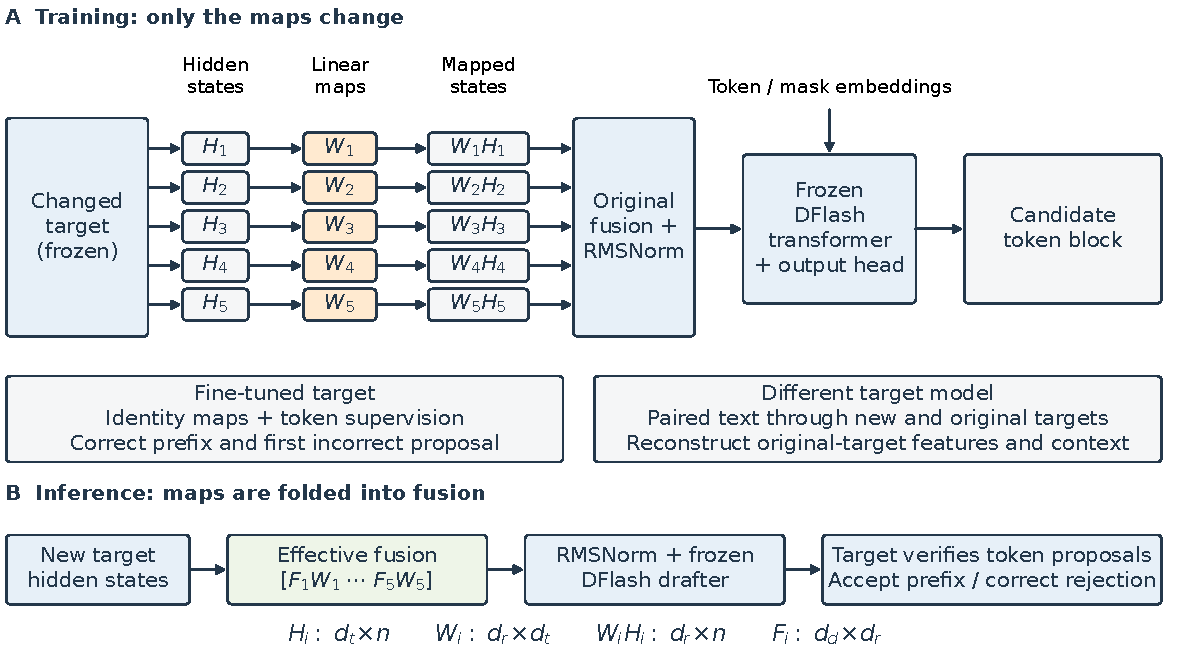
\includegraphics[width=\linewidth]{figures/relayspec_overview.pdf}
    \caption{RelaySpec training and inference. Orange maps are trainable and blue model components are frozen. Each hidden-state matrix $H_i$ enters a map $W_i$ before fusion. A single position gives the matrix--vector product $W_i h_{i,t}$. Here $n$ counts context positions, $d_t$ is the new target's feature width, $d_r$ is the width expected by the drafter, and $d_d$ is its hidden width. For Qwen3-8B with the Qwen3-4B drafter, $d_t=4096$ and $d_r=d_d=2560$. Each $W_i$ is $2560\times4096$, and exported fusion is $2560\times20480$. The new target verifies proposals after adaptation.}
    \label{fig:relayspec-overview}
\end{figure}

For a LoRA-fine-tuned target, identity initialization leaves its hidden states unchanged and preserves the existing drafter's behavior with that target. The maps therefore introduce no additional disruption at initialization. Training then modifies those hidden states so that they better condition the frozen drafter to predict the LoRA-adapted target's tokens. We use \emph{accept-until-fail (AUF)}: cross-entropy on saved target responses supervises the correct draft prefix and its first incorrect proposal~\citep{yang2026specauf}. Later positions are excluded because verification would stop at the earlier error.

For cross-model transfer, the drafter was trained to process hidden states from its original target. Replacing that target changes the features, and sometimes their dimensions, so the same drafter may no longer interpret them effectively. We run the original and new targets on the same text and train linear maps to reconstruct the original target's features from the new target's features. The \emph{mean squared error (MSE)} objective has two terms: one compares each mapped feature with its original-target counterpart, and the other compares their combined context after the frozen fusion projection and RMSNorm. The context term supervises what the draft layers actually receive, beyond matching each layer separately. Both terms use squared errors scaled by the corresponding original-target vector's squared norm, with numerical stabilization.

We evaluate specialization, cross-model transfer, training budgets, and shared serving. Matched comparisons include draft-body updates, direct fusion updates, and different token objectives. Their results delimit the method: body adaptation or decaying cross-entropy can be stronger on some workloads, and a pooled adapter can approach separate task adapters. We therefore measure both single-request and shared-serving performance rather than assume that every target needs a separate drafter or that higher acceptance always gives higher throughput.

We analyze the learned maps to understand why adaptation helps. First, we use singular value decomposition (SVD) to retain only the largest components of either the full map $W_i$ or its correction $\Delta_i=W_i-I$. For the tested GSM8K and NanoCoder checkpoints, truncating the full map to rank one or two sharply reduces acceptance. Using $I+[\Delta_i]_r$, where $[\Delta_i]_r$ is the rank-$r$ truncated correction, preserves more acceptance, though these low ranks do not recover the full-map result. Second, scaling only the correction shows that half strength retains much of the benefit, while stronger corrections reduce acceptance. Third, we compare the correction with the LoRA-induced change in fused hidden states. Their mean cosine similarities are close to zero and similar to shuffled-position controls, providing no evidence of systematic cancellation of the LoRA change. Finally, in cross-size transfer, moving token-trained maps halfway toward an MSE-trained solution improves acceptance and throughput on the tested Math and Code workloads. This supports learning inputs the frozen drafter can use, without establishing a universal advantage for MSE.

Our contributions are:
\begin{itemize}
    \item We propose RelaySpec, which adapts a pretrained DFlash drafter through five linear maps while freezing its transformer. The maps fold into the original fusion projection, and we study token supervision for target specialization and feature reconstruction for cross-model reuse.
    \item We evaluate adaptation across fine-tuned targets, model sizes, and families, including training-budget and shared-serving comparisons. On Qwen3-4B LoRA targets, the selected AUF maps improve mean per-request throughput over the unchanged DFlash drafter by 37.58\% and 89.52\% on GSM8K and KiCad, respectively. The selected Qwen3-4B-to-8B transfer recovers 100.2\% and 99.4\% of native-drafter throughput on MATH and GSM8K, with weaker transfer on code and chat.
    \item We analyze full-map and correction-map SVD truncation, correction scaling, alignment with LoRA-induced feature changes, and interpolation toward MSE-trained maps.
\end{itemize}
